%\section{Wprowadzenie}
\section{Introduction}

%Integracja technologii baz danych z nowoczesnymi metodami
%indukcyjnego generowania wiedzy jest naturalnym kierunkiem rozwoju
%system�w bazodanowych. 

The integration of the data base technology with modern inductive methods of
generation knowledge is a natural direction of a development databases system.

%Systemy nazywane czasem indukcyjnymi bazami
%danych potrafi� odpowiedzie� nie tylko na pytania, dla kt�rych
%odpowied� znajduje si� w bazie danych, ale r�wnie� na pytania,
%kt�re wymagaj� zsyntetyzowania i zastosowania wiedzy,
%wygenerowanej przez indukcyjne wnioskowanie z fakt�w z bazy danych
%i wcze�niejszej wiedzy~\cite{bib3}. 

Systems which are called inductive data bases allows finding answers on the questions,
for which replies are in the dat base and also on questions which demend 
synthetize and use knowladge generated by inductive deduction from facts from
database and earlier knowladge.


% Schemat typowej indukcyjnej
% bazy danych przedstawiony jest na rysunku~\ref{fig:inddb}.
A schema of a typical inductive data base was presented on the picture
~\ref{fig:inddb}.

\begin{figure}[!ht]
    \centering
        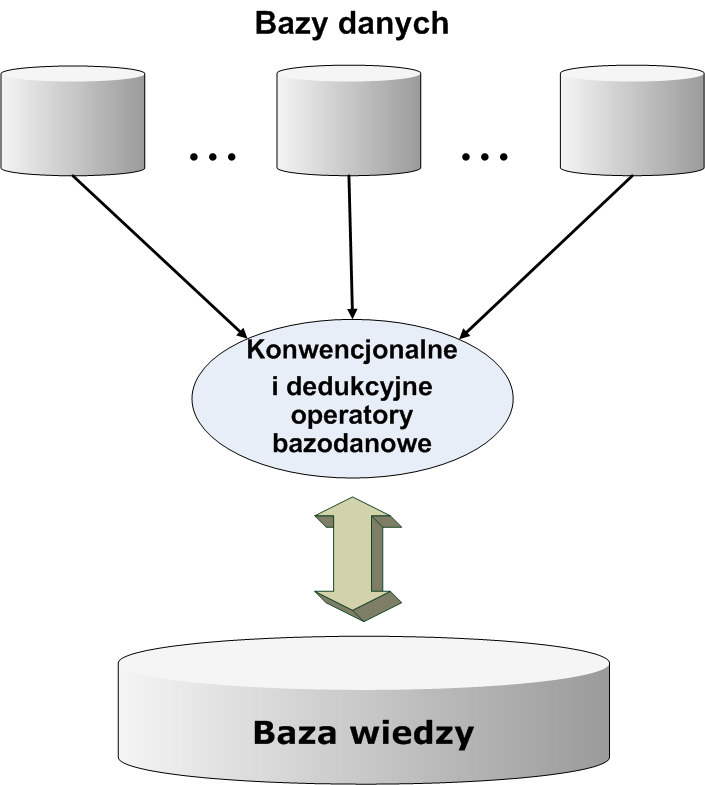
\includegraphics[width=\linewidth]{img/knowledge_mining.png}
%    \caption{Indukcyjna baza danych~\cite{bib2}}
    \caption{Inductive data base~\cite{bib2}}
    \label{fig:inddb}
\end{figure}



%W pierwszej cz�ci pracy przedstawione zosta�y wybrane istniej�ce
%�rodowiska wspieraj�ce uruchamianie algorytm�w uczenia maszynowego.
Selected enviroments which allow runing
algorithms of maching learning were described in the first part of the article.

%Dalej opisano za�o�enia, a~nast�pnie architektur� i wybrane aspekty
%implementacji komponentowej realizacji indukcyjnej bazy danych --
%platformy \emph{Salomon}.

Assumptions, the architecture and some of implementation aspects of component
realization of the inductive database -- the \emph{Salomon} platform were
described in the next part of the article.

%  Dzi�ki budowie modu�owej uda�o si� uzyska�
%du�o wi�ksz� elastyczno�� systemu w stosunku do opisanych wcze�niej
%rozwi�za�.

The last part of the article shows possibilities of using the platform to learn
decision treeies.
%  Ostatnia cz�� pracy prezentuje mo�liwo�ci wykorzystania
%platformy do uczenia drzew decyzyjnych.

Thanks to the modular structure much better system flexibility
in comparison to described below systems was achieved.

